%%% introduction.tex: -*- LaTeX -*-  DESCRIPTIVE TEXT.
%%%
%%% Copyright (c) 2017 Brian J. Fox & Orchid Labs, Inc.
%%% Author: Brian J. Fox (bfox@meshlabs.org)
%%% Author: A truckload of others
%%% Birthdate: Tue Oct 10 11:59:37 2017.

\subsection{System Goals}

The \Orchid{} Network was designed with three goals:

\begin{enumerate}
\item To codify the right to unrestricted, unsurveilled Internet access on a network level.
\item To build a system suited for daily use. To say that a freedom is not a part of daily life is to say that the freedom is dying.
\item To make such a system worthy of trust, by developing it in the open and releasing the source code for full public audit.
\end{enumerate}

These are ambitious goals, and are not realized by the system described in this document. This document does, however, contain an imperfect first attempt – an invitation to join us in design, construction, and use of what we believe is the future of networking.

\subsection{Acknowledgements}

We would like to extend special thanks to Professor Dan Boneh, Professor Paul Vigna, Justin Sheek, Brian Vohaska, and all of our early investors and advisors. Without their passion for this problem domain, and their willingness to take a risk chasing a solution, this project would not have seen the light of day.

\subsection{Terms}

\begin{itemize}
\item Node. A computer running a program which implements the \Orchid{} Protocol.
\item Medallion. Data used by a node to demonstrate it is in exclusive possession of computational resources.
\item User. The owner of a node.
\item Orchid Market. A P2P collection of nodes interacting through the \Orchid{} Distributed Marketplace Protocol.
\item \emph{The} Orchid Market. \TOM{} in possesion of the most global computational power.
\item Customer. A buyer on \tOM{}.
\item Peddler. A node who is a member of an Orchid Market's collection.
\item Entry Peddler. A Peddler who is willing to accept direct TCP connections from Customers.
\item Address. The location in Medallion-space inhabited by a Peddler.
\item Relay. A Peddler willing to sell bandwidth to customers.
\item Proxy. A Relay which is additionally willing to interact with web servers on behalf of Customers.
\item Chain. A list of n Relays ending in a Proxy used for anonymous communication by a Customer.
\item Ticket. A stochastic micropayment.
\item Attack. A method for causing the non-consensual transfer of money or information.
\item Attacker. A person or group of people interested in performing attacks.
\end{itemize}

\subsection{High-Level System Overview}

\subsubsection{\TOM{}}

\begin{figure}[htbp]
  \centering
  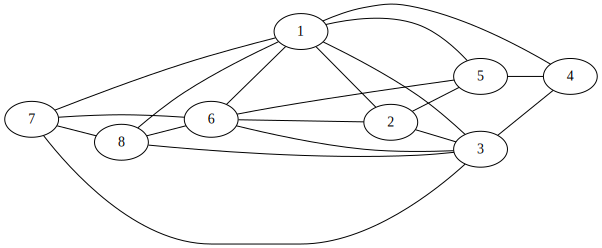
\includegraphics[width = 300pt]{marketOverview}
  \caption{An Orchid Market with eight Peddlers}
\end{figure}

\TOM{} is a globally distributed P2P market place for bandwidth. \TOM{} connects Peddlers to each other randomly, and has each Peddler verify the ``realness'' of its connected peers.

\subsubsection{Chains}

\begin{figure}[htbp]
  \centering
  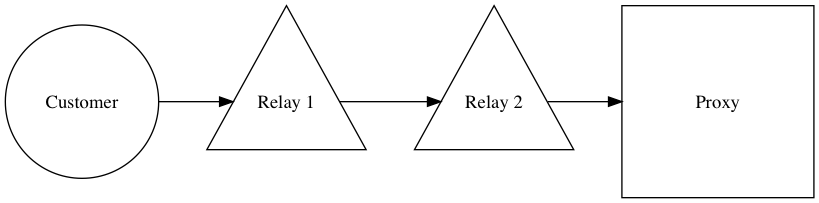
\includegraphics[width = 300pt]{sttc}
  \caption{A three-Peddler Chain routing traffic for a Customer}
\end{figure}

Once relay and proxy bandwidth has been purchased, the customer configures them into a directed acyclic graph termed a Chain. In the above picture, Relay 1 receives bandwidth from the Customer, performs cryptographic operations on it, and forwards the resulting data to Relay 2. Relay 2 performs a similar role with respect to Relay 1 and the Proxy. The Proxy then sends this data to a web server. Any data returned by the web server is sent back to the Customer along another chain, perhaps implemented using the same nodes in reverse.

\subsubsection{Web Browsing}

The majority of initial usage of the \Orchid{} Network will likely happen in support of uncensorable, anonymous web browsing. In this use case, the client software will automatically use \tOM{} to create a Chain, and provide additional checks to verify that SSL/TLS is being used in a way suited to this networking model. Unless two or more nodes in a Chain are working together (Section \ref{sec:collusion}), perhaps because they are run by the same user, no single node knows the Customer's IP Address and the server they communicated with.

\subsection{User Stories}

\subsubsection{Bandwidth Miners}

Users with excess computational power and bandwidth may choose to support the \Orchid{} Network, as well as earn money, by running a Peddler on their computer. To do so, they install and run the \Orchid{} software package and supply a payment address. To verify realness while preserving anonymity, the software will convert computational resources into Medallions. Peddlers are compensated for their lost computation by bandwidth consumers.

\subsubsection{Resisting Oppressive Governments}

Users who live under oppressive regimes (where, for example, it is illegal to access Wikipedia), can use the system to hide information about the websites they are browsing. To do so they install and run the \Orchid{} software, provide an initial payment to their \Orchid{} wallet, and browse the web as normal. Unlike similar services (Section \ref{sec:prior-work}), the network pays hosts for their participation. We hope this will lead to greater participation, which in turn will lead to grater anonymity (Section \ref{sec:market}).

\subsubsection{Resisting Oppressive Web Applications}

Users of oppressive web applications (sites which change services offered based on geographic location), can use the \Orchid{} Network to appear to be browsing from the country of their choice. Unlike similar services (Section \ref{sec:prior-work}), traffic will not come from IP ranges allocated to server farms, and so will be much harder for oppressive websites to block. Additionally, because bandwidth is incentivized, it will likely prove much more plentiful on the \Orchid{} Network, i.e. making the real-time playback of high resolution video viable.
